\documentclass{article}
\usepackage[margin=0.8in]{geometry} % change this parameter to enlarge/restrict the margins
\usepackage{amsmath,amsthm,amssymb,amsfonts, fancyhdr, color, comment, graphicx, environ}
\usepackage{xcolor}
\usepackage{mdframed}
\usepackage[shortlabels]{enumitem}
\usepackage{hyperref}
\usepackage{calrsfs}
\DeclareMathAlphabet{\pazocal}{OMS}{zplm}{m}{n}
\usepackage{graphicx}
\usepackage{makecell} %table cells
\usepackage{booktabs} %table appearance
\usepackage{caption} %table caption


\renewcommand{\footrulewidth}{0.8pt}
\hypersetup{
	colorlinks=true,
	linkcolor=blue,
	filecolor=magenta,      
	urlcolor=blue,
}

%/ Margin
%/ ##########################
%/\addtolength{\oddsidemargin}{-.7in}
%/\addtolength{\evensidemargin}{-.7in}
%/\addtolength{\textwidth}{1.4in} %/Double of the 2 above
% ###########################

% fancy style 
\pagestyle{fancy}
% remove fancy style from bottom 
\renewcommand{\footrulewidth}{0pt}

\lhead{Daniele Falcetta, Simone Papicchio, Massimiliano Pronesti, Federico Tiblias}
\rhead{AML} 

\newcommand{\loss}{L(\theta, a)}
\newcommand{\lossRule}{L(\theta, \delta(x))}
\newcommand{\risk}{R(\theta, \delta)}

%------------------------------------------------
%% Bibliography
%\usepackage[sorting=none, backend=bibtex]{biblatex}
%\addbibresource{ref.bib}
%------------------------------------------------

\begin{document}
	\title{\Large Algorithmic Machine Learning  \\[0.5cm]
	\bf\Large Challenge 1 - Report \\[0.5cm]
	
	\bf\Large Group 20}

\author{\large 
	\begin{tabular}{rl}
		\textbf{Professor:} & Pietro Michiardi \\
		\textbf{Authors:} & Daniele Falcetta \\ & Simone Papicchio \\ & Massimiliano Pronesti \\ & Federico Tiblias
	\end{tabular}
	}
\date{\large \today}

\makeatletter
\begin{titlepage}
	\begin{center}
		{ 
\includegraphics[width=10cm]{assets/eurecom.png}}
		{\ \\ \ \\}
		\vbox{}\vspace{5cm}
		{\@title }\\[3cm]
		{\@author}\\[3cm]
		{\@date\\}
		
	\end{center}
\end{titlepage}
\makeatother
	
\section{Introduction}
    The Weather Forecast problem consists in using climatic measurements and predictions from different models (Global Forecast System, Global Deterministic Forecast System from the Canadian Meteorological Center, Weather Research and Forecasting) in order to predict the air temperature measurement at 2 metres above the ground. The dataset shows highly correlated features and a serious shift between train and test distributions.
    When the distribution of the train and test data differs, this is known as dataset shifting. This may cause several problems because the model is trained on one distribution but is used to make predictions on a different one, resulting in poor results. There are different types of data shifting such as 
    Covariance Shift\footnote{Changes in the independent variables or features of the dataset},
    Probability Shift\footnote{Changes in the target variable or the dependent variable in the dataset}
    and Concept Shift.\footnote{Change in the connection between the independent and the target variable across datasets}
    In this work we analyze the presence of the Spatial Covariance Shift and try to address its main challenges.

    The data represents pairs of meteorological features and target values at a particular latitude/ longitude and time. The Regression task consists in predicting the air temperature measurements at 2 meters above the ground.
    The features are either direct measurements (such as sun elevation at the current location, humidity, temperature, pressure and topography, and other meteorological parameters) or weather predictions provided by climatic models (Global Forecast System, Global Deterministic Forecast System from the Canadian Meteorological Center, Weather Research and Forecasting).
    Each model returns the following predicted values: wind, humidity, pressure, clouds, precipitation, dew point, snow depth, air and soil temperature characteristics. Where applicable, the predictions are given at different isobaric levels from 50 hPa (20 km above ground) to the ground level.
    Altogether, there are 111 features in total. It is important to note that the features are highly heterogeneous, i.e., they are of different types and scales.
    The main challenge of this dataset is the handling of the Spatial Covariance Shift from train to test as visible in Fig. \ref{fig:train-test-diff}

    \begin{figure}[h]
        \centering
        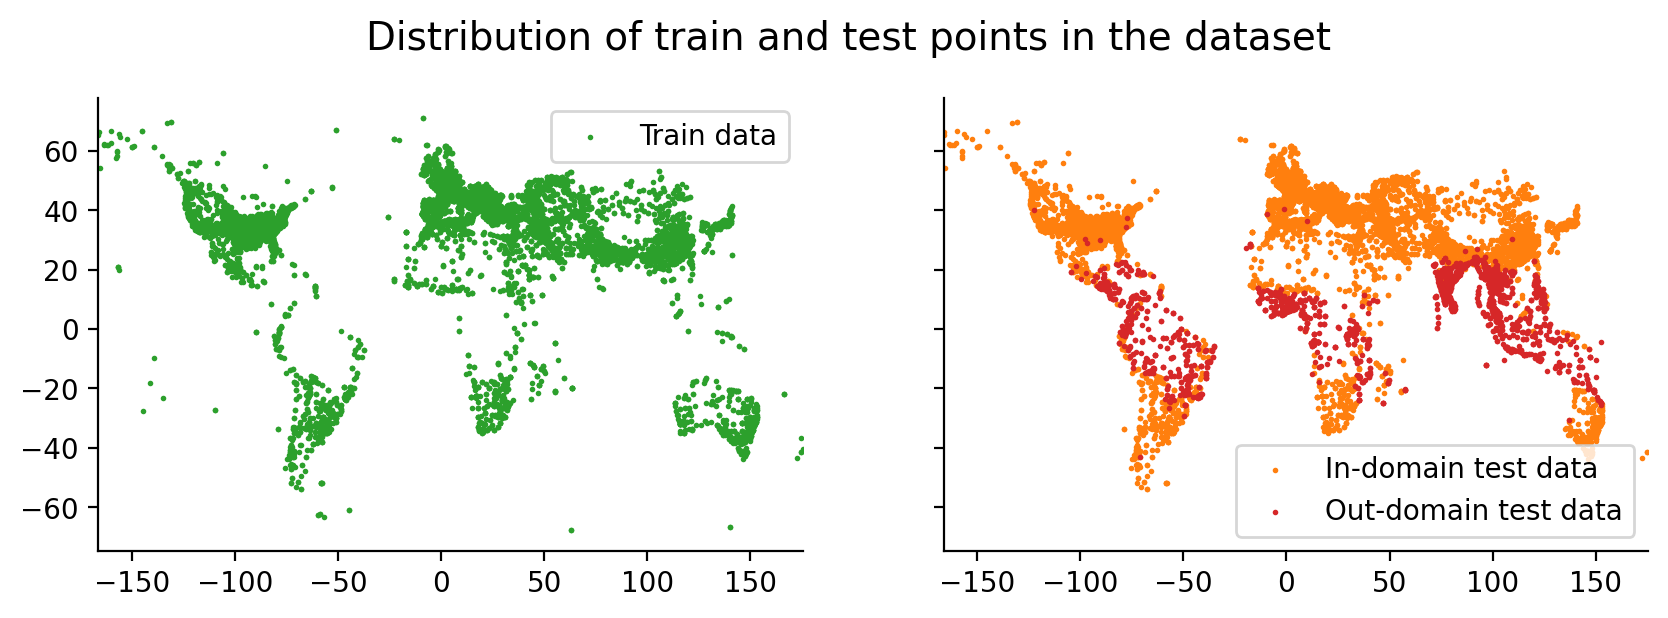
\includegraphics[width=\linewidth]{assets/train-test-diff.png}
        \caption{The figure clearly shows that the regions in the range of latitude from -18 to 10 are not present in the train dataset. This phenomenon is called \textit{Spatial Covariance Shift}. [best visualization in colors] }
        \label{fig:train-test-diff}
    \end{figure}

\section{Data Analysis}
    \subsection{Outliers}
    The first step of our dataset analysis focuses on the outliers detection. Our approach, based on the Interquartile method (IQR), consists in plotting a boxplot for each feature. To obtain better and more organized visualizations, we opted for plotting four different graphs, one for each weather forecast model and, given the high heterogeneity of the features, we scaled our data between 0 and 1 according to a min-max normalization. This analysis shows that almost all the features contain some outliers. In Section 4 we show some experiments attempting to remove part or all of them. A particular mention has to be done for the feature \textit{gfs\_soil\_temperature}, which contains some entries equal to -9999 °C, i.e. a missing measurement, as reported in the associated feature \textit{gfs\_soil\_temperature\_available}.
    
    
    
    \subsection{Correlations}
    An important element of the analysis is understanding the correlations present in the dataset. We start analyzing the correlation between the features and the target. Table 1 shows the ten features that correlate most with the target. An approximate analysis would lead to the removal of all the other features. However, there are two problems with this approach. First, the Pearson coefficient analyzes only linear correlations, it does not take in consideration non linear ones. Second, we are not considering that features can correlate between each other. If high correlation is present between two features they carry the same information and one of them can be dropped. Indeed, we discover that the \textit{gfs\_temperature\_xxxxx} are correlated when they are in similar conditions\footnote{The temperature measurements are taken in close isobaric levels}. The same kind of correlation can be detected among other groups of features. To address both issues, we perform feature selections by means of the feature importances returned from the Random Forest\footnote{n\_estimators=10, max\_depth=25}.  
    
    \subsection{Feature Shift}
    Train and test datasets show a noticeable shift in the distribution of samples: test datapoints are distributed homogeneously around the globe, while the train dataset lacks samples in the equatorial region. To gain a deeper understanding of how this phenomenon affects our prediction we compute a metric reminiscent of the Wasserstein distance. For each feature we divide the dataset into 100 bins of equal size and normalize them in order to obtain histograms. Then, we compute the area difference between the cumulative sum of these histograms for train and test datasets. The value we obtain represents some notion of distance between the two distributions and can be used later on during feature selection. We report in Table 2 the 10 most shifted features according to this metric. 

\vspace{0.5cm}    
\setlength{\tabcolsep}{8pt}
\hspace{-0.5cm}\begin{minipage}[c]{0.5\textwidth}
\centering
\begin{tabular}{lccl}
\toprule
\makecell{Feature}                         & \makecell[t]{Pearson\\ Correlation} \\ \midrule
\textbf{wrf\_t2\_interpolated}   & \textbf{0.963}     \\
wrf\_t2\_next                   & 0.958               \\
gfs\_temperature\_97500         & 0.874               \\
gfs\_temperature\_95000         & 0.863               \\
climate\_temperature            & 0.857               \\
gfs\_temperature\_92500         & 0.852               \\
gfs\_temperature\_90000         & 0.842               \\
gfs\_temperature\_85000         & 0.824               \\
gfs\_temperature\_80000         & 0.808               \\
cmc\_0\_0\_6\_2                 & 0.807               \\ \bottomrule
\end{tabular}
\captionsetup{width=0.8\linewidth}
\captionof{table}{Features most correlated to target value in the training dataset according to Pearson metric.} %\ 
\end{minipage}
\begin{minipage}[r]{0.5\textwidth}
\centering
\begin{tabular}{lccl}
\toprule
\makecell[c]{Feature}                         & \makecell[t]{Wasserstein\\ distance} \\ \midrule
fact\_latitude                  & 13.625               \\
gfs\_total\_clouds\_cover\_high & 13.718               \\
gfs\_temperature\_15000         & 14.541               \\
gfs\_v\_wind                    & 16.866               \\
gfs\_precipitable\_water        & 16.999               \\
cmc\_0\_1\_0\_0                 & 17.057               \\
gfs\_2m\_dewpoint\_grad         & 24.006               \\
cmc\_available                  & 49.000               \\
gfs\_available                  & 49.000               \\
\textbf{wrf\_available}                  & \textbf{49.000  }             \\ \bottomrule
\end{tabular}
\captionsetup{width=0.8\linewidth}
\captionof{table}{Most shifted features between train and test datasets according to Wasserstein metric.}
\end{minipage}

%\begin{table}
%\begin{center}
%\begin{tabular}{lccl}
%\toprule
%Feature                         & Wasserstein distance \\ \midrule
%fact\_latitude                  & 13.625               \\
%gfs\_total\_clouds\_cover\_high & 13.718               \\
%gfs\_temperature\_15000         & 14.541               \\
%gfs\_v\_wind                    & 16.866               \\
%gfs\_precipitable\_water        & 16.999               \\
%cmc\_0\_1\_0\_0                 & 17.057               \\
%gfs\_2m\_dewpoint\_grad         & 24.006               \\
%cmc\_available                  & 49.000               \\
%gfs\_available                  & 49.000               \\
%wrf\_available                  & 49.000               \\ \bottomrule
%\end{tabular}
%\end{center}
%\captionof{table}{Most shifted features between train and test dataset according to Wasserstein metric.} 
%\end{table}


    \section{Pre-Processing}
    Different models call for different preprocessings and feature selections. We try different approaches in conjunction with one or more models to find the best one in each situation.
    \begin{itemize}
        \item \textbf{Dealing with missing values:} either fill missing values with their respective column mean or drop samples containing at least one NaN.
        \item \textbf{Outlier removal} either use the interquartile method or the local outlier factor.
        \item \textbf{Rescaling:} normalize all features using sklearn's \textit{StandardScaler}.
        \item \textbf{Feature selection based on Random Forest feature importance:} train a Random Forest to predict the target value and  keep only the $n$ most important features according to the model. Use these selected features with another model.
        % Fill in the others.
        \item \textbf{Feature selection based on Wasserstein distance:} rank features according to the metric described in the previous section and keep only the $n$ less shifted ones as they should better represent the test distribution.
        \item \textbf{PCA:} correlation analysis shows many features are correlated, this poses a problem for linear models. We address this issue by performing a PCA keeping either \textit{num\_features} - 1 principal components or by selecting the components explaining $99\%$ of variance.
        \item \textbf{Daylight and hour:} use \textit{fact\_time, fact\_latitude, fact\_longitude} to compute amount of daylight received and hour the measurement took place.
    \end{itemize} 
    %Rivedere i tempi verbali?
    
    \section{Models}
    We perform an initial exploratory analysis comparing a variety of models along with different preprocessings and pick the ones that perform best to be further explored with hyper-parameter tuning. 
    
    The models we compared are:
    \begin{itemize}
        \item \textbf{Ridge:} Gives promising results but is susceptible to collinearity. PCA is always required to train it. Removing most shifted features seems to positively affect performances.
        \item \textbf{Random Forest:} Robust to outliers, it gives good performance for a small number of estimators. The downside is its training time.
        \item \textbf{Catboost:} Performs very well without any feature selection or PCA required. Being an ensemble method it is much more difficult to interpret, training takes a long time.
        %Possiamo spiegare di più?
        \item \textbf{Gradient boosting regressor:} Same issues as Catboost but we observe worst performances.
        \item \textbf{Support vector regressor:} Training takes an unfeasible amount of time.
    \end{itemize} 
    
    \section{Hyper-parameter tuning}
    We decide to not split the dataset in train and test since the retraining of the best model was more computationally expensive then running the CV. Consequently, in order to avoid the model to learn statistics from the validation samples, we create a Pipeline\footnote{sklearn.pipeline.Pipeline} which is fitted on the train folds and used on the test fold. In this way, we were able to analyze the performance of the model on a dataset never seen before.
    Since different models need different preprocessing, we define different pipelines. Then for each model we use a simple Grid Search with five cross validation. We do not investigate more complex technique such as RandomGridSearch or HalvetGridSearch because due to the huge time complexity needed for training, we tuned our models on a small amount of hyperparameters. In Table 3 are shown the results.
    
    
\setlength{\tabcolsep}{1.7em}
\begin{table*}[t]
\centering
\begin{tabular}{p{2cm}p{3.3cm}p{2.3cm}p{1cm}p{1cm}}
\toprule
%THESE ARE ONLY PLACEHOLDER VALUES, FILL IN CORRECT ONES
\makecell[t]{Preprocessing \\\& Model} & \makecell[t]{Hyperparameters \\explored} & \makecell[t]{Best \\hyperparameters} & \makecell[t]{Validation \\score} & \makecell[t]{Test score \\(Kaggle)}\\ \midrule
\makecell{StandardScaler,\\ PCA, Ridge} & \makecell{alpha: [0.1, 0.01, 0.001]} & \makecell{alpha: 0.1} & \makecell[t]{\\0.420} & \makecell{\\0.690}\\
\makecell{StandardScaler, \\Random Forest }&  \makecell{num\_iterations: [10, 25, 20] \\ max\_depth: [3, 6, 9]} &  \makecell{num\_iterations: 10 \\ max\_depth: 3} & \makecell{0.420} & \makecell{0.690}\\ \bottomrule
\end{tabular}
\captionof{table}{Models and hyperparameters tested.} 
\end{table*}
    
\section{Results}
By applying different combinations of preprocessing we observe the following:
\begin{itemize} 
    \item Filling missing values with the column mean or dropping the sample altogether produces comparable results. We choose to always fill with the mean to avoid dropping potentially useful samples.
    \item Although we try different outliers removal techniques over distinct experiments, we obtain our best results by keeping the outliers in the analysis.
    \item Rescaling proves always useful in improving performances.
    \item Despite our efforts in coming up with sensible metrics for feature selection we find that keeping all features and letting the model choose the most important ones during training is still the best-performing approach despite the presence of spatial shift. It looks like the features
    \item PCA is needed only for linear models to avoid collinearity. Other models show a reduction in performance when PCA is applied.
    \item Daylight and hour do not lead to any noticeable improvements on any analyzed model. 
\end{itemize} 

Regarding the models, we observe that Ridge performs well enough and is a rather simple model to train. The best results were obtained for XXX and YYY.
%\Completare
Catboost proves to be the best performing method

These results suggest that this dataset hardly requires any preprocessing or feature selection. The highest scoring methods either perform regularization or implicit feature selection thanks to trees, showing that an automatic choice of features wins over a curated manual one. This does not surprise us: plenty of features correlate extremely with the target and require no fancy transformation to be used effectively by the models.

\section{Conclusions}
We show a simple way Catboost can be used to predict temperature measurement with very little preprocessing required. This solution though simple yields good results.
%Future works
Our model does not apply any transformation to the data and is thus limited to a linear representation. This work could be expanded by also considering polynomial features, looking for higher degree relationships.

Despite consisting of almost 2 million measurements, the actual weather stations are few in number, totaling around 5000. A more detailed analysis could investigate aggregates of measurements coming from the same station in order to increase performance. An even more refined approach would be to group together measurements coming from the same station and treat the prediction as a time series problem, applying models such as RNNs and LSTM.
 %/ General comment secondo me ==> Evitare le forme contratte "it's" o "doesn't"
%%%%%%%%%%%%%%%%%%%%%%%%%%%%%%%%%%%%%%%%%%%%%%%%%%%%%%%%%%%%%%%%%%%%%%%%%%%%%%%%


\end{document}